%% IEEE conference version of the paper.
%% Sections I--III: Introduction, Related Work, Method. Chapter 3 of the thesis holds the full method.
%% Compile: pdflatex, bibtex, pdflatex, pdflatex.
\documentclass[conference]{IEEEtran}
\usepackage[T1]{fontenc}
\usepackage[utf8]{inputenc}
\usepackage{cite}
\usepackage{amsmath,amssymb,amsfonts}
\usepackage{graphicx}
\usepackage{textcomp}
\usepackage{xcolor}
\usepackage{url}
\usepackage{array}

% IEEEtran leaves 0.2ex of stretch in \parskip; with \flushbottom that
% stretch turns into visible blank lines when a column ends short.
\setlength{\parskip}{0pt}

\title{Persona-Based Multi-Agent LLM Debate as an Automated Playtester:
Validating Game Difficulty Data Against Human Performance Baselines}

\author{\IEEEauthorblockN{Muhammad Haydar Maulana}
\IEEEauthorblockA{Master of Informatics\\
Email: haydariday@gmail.com}}

\begin{document}

\maketitle

\begin{abstract}
Large language model (LLM) agents can estimate game difficulty far more cheaply than manual playtesting. The playtesters reported so far use a single agent with one playstyle. It is therefore unclear whether their estimates stay consistent across runs or reflect the population a designer cares about. This paper presents a persona-based multi-agent LLM debate playtester. A Game Master and three advisors with distinct Wordle playstyles debate each guess before the Game Master plays it. Three conditions are compared: the persona debate, a single agent and a debate without personas. Each plays 100 Wordle puzzles ten times under one configuration, against the public human results for the same puzzles. At the puzzle mean the debate repeats its estimates, with an ICC(1,10) of 0.91. It ranks the puzzles in line with human difficulty at $\rho$ from 0.69 to 0.75. The debate without personas is the most consistent condition, with a within-puzzle SD of 0.50 against 0.64 for the single agent. The personas raise that spread. The personas change how the playtester plays, raising the share of guesses that rule out letters from 5.6\% to 79.2\%, without improving agreement with human difficulty. A single agent therefore gives an equally good ranking for a twelfth of the output tokens, so the debate buys stability rather than accuracy.
\end{abstract}

\begin{IEEEkeywords}
automated playtesting, game difficulty, large language models, multi-agent debate, persona, Wordle
\end{IEEEkeywords}

\section{Introduction}
\label{sec:introduction}

Game designers need to know whether a game is hard enough for its intended players \cite{weber2020}. A game that is too hard drives players away, while one that is too easy soon becomes stale, both of which risk a negative reception \cite{karavidas2022}. Difficulty is therefore tied to player engagement and experience \cite{romero2023,alvarado2021}. Designers measure it through playtesting. However, manual playtesting is resource-intensive, since it needs many testers over many sessions and must be repeated after every significant design change \cite{weber2020,prasetya2026,zhao2025}. For indie developers with limited budgets, this cost is often prohibitive.

Automated playtesting offers an alternative. Hand-crafted methods, such as programmed test agents \cite{prasetya2026} and mathematical difficulty models \cite{francillette2025}, require substantial engineering for each game. Learning-based methods need large training resources and tend to play in ways that humans would not \cite{delfosse2025}. Large language model (LLM) agents avoid both costs, since they play games such as chess \cite{feng2023}, Pok\'emon battles \cite{hu2024} and Minecraft \cite{wang2023} from a text description of the rules. Xiao and Yang \cite{xiao2025} show that the difficulty LLM agents experience in Wordle and Slay the Spire follows that of human players, even though the agents play worse.

These LLM playtesters still rely on a single agent with one playstyle, while human players differ, since some take risks while others play safely. Gameplay data from a commercial title also reveals distinct behavioral player types \cite{drachen2009}. Multi-agent systems also replicate human strategic behavior more closely than single LLMs do \cite{sreedhar2025}. It is therefore unclear whether an LLM playtester can produce data that is both consistent across runs and aligned with human players once several playstyles are considered.

To address this gap, this paper builds a persona-based multi-agent LLM debate playtester that combines playstyle personas \cite{holmgard2019} with multi-agent debate \cite{liang2024}. A Game Master (GM) and three advisors with playstyles Bold, Cautious and Casual debate each guess, after which the GM decides the action to play. Difficulty comes from the outcome of each playthrough, such as the number of guesses used, which is compared with human performance baselines on the same puzzles \cite{constant2017,xiao2025}. Wordle serves as the case study because its games are short, its feedback is deterministic and public per-puzzle human results are available.

The study asks two questions. RQ1: how consistent are the playtester's outcomes across repeated runs on the same puzzles? RQ2: to what extent do the resulting difficulty estimates agree with human difficulty, measured by average guess scores and difficulty categories? In addition, the study describes how the personas behave during the debate and how often their suggestions reach the final guess. For game developers, this indicates whether an LLM playtester can supply difficulty data that reflects human players, which would reduce their reliance on manual playtesting.


\section{Related Work}
\label{sec:related}

\subsection{Automated Playtesting}
Playtesting observes how players experience a game under development, so designers can find faults and levels that are harder than intended \cite{weber2020}. Manual playtesting is resource-intensive, since it needs many testers over many sessions and must be repeated after every design change \cite{prasetya2026,zhao2025}. Automated playtesting replaces these testers with software agents that play the game and record each playthrough. An agent costs only tokens and time, so the same puzzle can be played many times, which no manual session can afford.

Automated methods differ in what they cost to build and how closely they resemble human play. Scripted agents and mathematical models offer the most control. Prasetya et al. \cite{prasetya2026} build controlled test agents from goal structures and domain-specific languages, which requires significant programming effort and a steep learning curve. The difficulty model of Francillette et al. \cite{francillette2025} needs no sophisticated AI, yet it covers only platformer games and demands a complex setup. Learned agents shift the effort to data and training instead. Gudmundsson et al. \cite{gudmundsson2018} train a network on human moves before it can predict the difficulty of new levels. Deep reinforcement learning agents learn from their own play, yet they need substantial training resources and lack the behavioral patterns of human play \cite{delfosse2025}. Procedural personas come closer to human play, since Holmgård et al. \cite{holmgard2019} tune agents to different playstyles, although each persona still relies on heuristics evolved for one game.

LLM agents avoid game-specific training, since they receive the rules and the current game state as text \cite{xiao2025}. Zhao and Tang \cite{zhao2025} convert the board of a match-3 game into numerical representations, after which their playtester reaches strong code coverage and detects bugs. Bateni and Whitehead \cite{bateni2024} show that LLM agents in Slay the Spire plan over the long term without specialized training. Xiao and Yang \cite{xiao2025} show that the difficulty LLMs experience in Wordle and Slay the Spire follows that of human players, even though the agents play worse. This study builds on that line, since LLM agents need neither per-game code nor training data. It asks whether their difficulty estimates hold when several playstyles take part.

\subsection{Difficulty and Behavioral Measures}
Constant et al. \cite{constant2017} distinguish subjective from objective difficulty. Subjective difficulty is how hard players perceive a game to be, while objective difficulty is the part that can be quantified without their perception. Subjective difficulty cannot be measured directly, since it depends on skill, stress and emotion. This study therefore uses objective difficulty. It is measured through behavioral performance measures, such as whether a challenge is completed, how many attempts it takes and how long it takes \cite{weber2020,romero2023}.

In Wordle, difficulty is measured by the guess count, so lower counts indicate easier words. Public per-puzzle results from real players\footnote{Engaging Data, ``Wordle Guess Distribution,'' \url{https://engaging-data.com/wordle-guess-distribution/}.} provide the average guess count of each puzzle, which is the human performance baseline, as in \cite{xiao2025}. Comparing a playtester with this baseline raises two questions. The first is whether the playtester gives similar outcomes when it plays the same puzzle again, since one run of an LLM may not represent its typical play. Xiao and Yang \cite{xiao2025} play each puzzle 20 times yet report only the average outcome, so this question remains open. The second is whether its outcomes rank and group puzzles as the human results do. Both comparisons are made per puzzle, because the baseline describes the player population rather than individual players. Both questions are addressed for the playtester built here.

\subsection{Personas and Multi-Agent Debate}
LLM agents can play diverse games, such as chess \cite{feng2023}, Pokémon battles \cite{hu2024} and Minecraft \cite{wang2023}, yet they play to win rather than to play like humans. Playtesting needs outcomes that resemble human play instead. Current LLM playtesters measure difficulty with a single agent that has one playstyle \cite{xiao2025}, or vary the personality of a testing agent to raise coverage, as MIMIC does \cite{chen2025}. Neither approach turns several playstyles into a difficulty estimate. Sreedhar and Chilton \cite{sreedhar2025} show that multi-agent systems replicate human strategic behavior more closely than single LLMs do. Before LLMs, Holmgård et al. \cite{holmgard2019} had already represented different players through procedural personas.

A persona is meant to change how an agent plays, but the evidence is mixed. Role-play prompting improves zero-shot reasoning on most of the twelve benchmarks \cite{kong2024}. In system prompts, personas do not improve accuracy on factual questions. The effect of a given persona can be largely random \cite{zheng2024}. In a strategic game, personas help only when a mediator translates them into heuristic values \cite{licato2025}.

Debate combines several agents into one decision. Agents propose answers and then revise them over rounds after reading the others, which improves factual accuracy and reasoning over a single agent \cite{du2024}. Liang et al. \cite{liang2024} have agents argue in a state of ``tit for tat'', each responding to the position before it, with a managing agent reaching the final decision. ChatEval \cite{chan2024} gives the debaters different roles and finds that the diversity matters. However, homogeneous debates often fail to beat single-agent chain-of-thought or self-consistency at matched compute \cite{zhang2025}. Their benefit also depends heavily on the setup \cite{smit2024}. Personas can drift too, as debating agents conform to their peers or abandon their assigned views \cite{baltaji2024}. None of these studies measures whether personas or debate improve difficulty estimates over a single agent.

Unlike studies that compare multi-agent systems with a single agent \cite{sreedhar2025,smit2024}, this study builds a playtester on the debate and validates it as a system. Agents with different playstyles argue over each guess, so the guess reflects more than one way of playing. The study then measures how consistent the outcomes are, how well they agree with human difficulty and how the personas behave. Whether the debate makes those measurements more stable, rather than merely different, is what the experiment tests.

\section{Method}
\label{sec:method}

\subsection{The Playtester}
The playtester has three parts around the game under test, which are the bridge, the multi-agent debate and the game knowledge (Fig.~\ref{fig:architecture}). In each turn, the bridge converts the public game state into text, since an LLM cannot see the board \cite{zhao2025}. The GM and three advisors then debate the next guess, after which the GM decides what to play. The bridge validates that guess and plays it in the game, while the feedback becomes the state of the next turn.

\begin{figure*}[t]
\centering
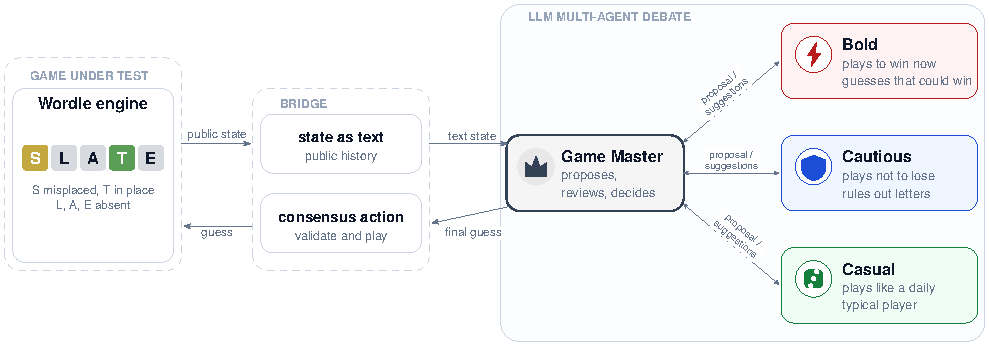
\includegraphics[width=\textwidth]{figures/fig-architecture.pdf}
\caption{The persona-based debate playtester. The game under test is external and drawn with a dashed edge, while the bridge passes the state and the guess.}
\label{fig:architecture}
\end{figure*}

The bridge renders the history of guesses as a keyboard-style letter summary, which plays the role of the colored keyboard that a human player sees. It lists the confirmed, misplaced and absent letters without any list of candidate words. The answer word, the guess limit and the human results never enter a prompt, so the playtester cannot copy the difficulty that it is measured against. The bridge accepts a guess only if it is an unplayed word from the 14,855-word allowed list \cite{atkins2022}. Every agent also receives the same game knowledge, which holds the rules, the reply format and its own persona instruction.

Three personas cover the ways that a player can spend a guess. Bold plays to win now and prefers guesses that could still be the answer, even at the risk of using more guesses later. Cautious plays not to lose and prefers guesses that rule out the most remaining letters, even if they cannot be the answer. Casual plays like a typical daily player, who picks familiar words without computing letter statistics. The GM holds no playstyle, since its role is to weigh the three arguments and to keep or revise the proposal. One advisor per playstyle is used, because debates with three agents already show clear gains \cite{du2024} and longer debates make agents lose track of the views of the others \cite{liang2024}.

These descriptions are condensed from the agents' instructions. Each agent is a zero-shot LLM call. The system message holds its instruction and the JSON schema of the reply, while the user message holds the public state and the task of the turn. The Cautious instruction, for example, opens with ``You are the Cautious advisor in a Wordle playtesting system'' before stating its playstyle.

\subsection{Debate Protocol}
The protocol has a managing agent oversee an exchange between the other agents \cite{liang2024}. The GM proposes a guess, after which each advisor reads the proposal and the transcript of the earlier rounds. Under the parallel rule, an advisor does not see the advice that the others give in the same round, so the three advisors of a round answer independently. Each advisor agrees with the proposal or suggests another word with a short reason. The GM reviews every suggestion and keeps or revises its guess, which ends the round. A new round starts from the first advisor, while the GM may stop early once another round is unlikely to change its decision.

The same rule appears in debates where agents read the others only from the previous round \cite{du2024}. It also keeps the speaking order out of the debate. A sequential rule would let each advisor read the suggestions of the same round. An advisor could then copy an alternative that an earlier one named, which would tie each persona to its position in the order. A turn allows at most three rounds, while an invalid reply is repaired up to twice. Every reply is a structured decision with an action, a reason and a stop flag.

\subsection{Experimental Configuration}
The three conditions differ only in the agents that decide each guess (Table~\ref{tab:conditions}). C1 is the full playtester of Fig.~\ref{fig:architecture}. C2 plays the game with one agent, as the single-agent playtesters of Xiao and Yang do \cite{xiao2025}. Its request holds only the game state and its task, while its game knowledge, bridge output and reply format stay the same. C3 keeps the GM and the three advisor slots, while the three advisors share one instruction with no playstyle. The difference between C3 and C2 therefore isolates the debate, since neither condition uses playstyles. The difference between C1 and C3 isolates the personas, since both conditions hold the same debate.

\begin{table}[t]
\caption{The three conditions. Only the agents that decide each guess differ.}
\label{tab:conditions}
\centering
\footnotesize
\begin{tabular}{@{}>{\raggedright\arraybackslash}p{0.50in}
>{\raggedright\arraybackslash}p{0.82in}
>{\raggedright\arraybackslash}p{0.68in}
>{\raggedright\arraybackslash}p{0.82in}@{}}
\hline
 & \multicolumn{1}{c}{C1} & \multicolumn{1}{c}{C2} & \multicolumn{1}{c}{C3} \\
\hline
Agents & GM + 3 advisors & one agent & GM + 3 advisors \\
Advisors & Bold, Cautious, Casual & -- & shared neutral text \\
Per turn & up to 3 rounds & one decision & as in C1 \\
Isolates & the full system & the reference & the personas \\
\hline
\end{tabular}
\end{table}

\begin{figure*}[t]
\centering
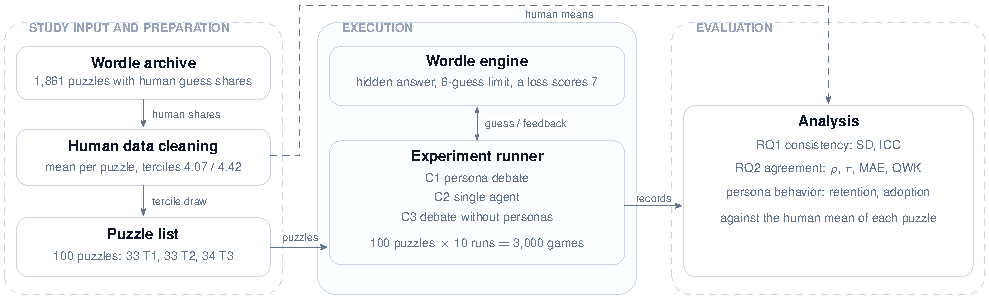
\includegraphics[width=\textwidth]{figures/fig-pipeline.pdf}
\caption{The study pipeline. The three conditions play one puzzle list, while the analysis compares their records with the human mean of each puzzle.}
\label{fig:pipeline}
\end{figure*}

All three play the same 100 puzzles with ten runs each, which gives 3,000 games and pairs every comparison by puzzle (Fig.~\ref{fig:pipeline}). The puzzles come from the public Engaging Data archive of past Wordle puzzles. Four of its 1,865 puzzles have missing data, which leaves 1,861 with a human mean. The share of players who did not solve a puzzle in six guesses is read as a loss scored 7, so every puzzle has a seven-bin distribution and a mean. The puzzles are sorted by mean and cut at 4.07 and 4.42 guesses into three equal terciles, T1 to T3 from easiest to hardest. The draw and the agreement measure then use the same three categories. The draw takes 33 puzzles at random from T1, 33 from T2 and 34 from T3. The hundredth puzzle goes to T3, which spans the widest range of means.

Each game ends within six guesses, while a loss is scored 7 to match the human data. The agents never see this limit, the answer word or any human result. Every condition runs on DeepSeek-V4.1-Flash with thinking enabled, a low reasoning effort, a reply limit of 8,192 tokens and JSON mode. The settings, the prompts and the limit were frozen before the first game, so every game uses one configuration. All 3,000 games completed under one code revision and one model snapshot.


\section{Results}
\label{sec:results}

The three conditions solved 99.7\%, 97.6\% and 99.6\% of their games within six guesses, at a mean score of 3.82, 3.87 and 3.83. The human mean of the same 100 puzzles is 4.30. The three conditions differ by at most 0.05 guesses, which is smaller than the gap to the human mean. The single agent solves slightly fewer games, though by under three games in a hundred.


\subsection{Consistency (RQ1)}
Table~\ref{tab:results} gives both families of measures. ICC(1,1) is the share of score variance that comes from the puzzle rather than from run-to-run noise. ICC(1,10) is the same quantity for the mean of ten runs. A single game carries only moderate information about its puzzle, since ICC(1,1) is 0.51 in the two debate conditions and 0.60 without personas. The mean of ten runs is highly reproducible, with ICC(1,10) of 0.91, 0.91 and 0.94, so the estimate that a designer would use repeats within a narrow interval.

\begin{table}[t]
\caption{Consistency and agreement with human difficulty. A better playtester has higher ICC and $\rho$ and lower SD and MAE. The best value in each row is in bold.}
\label{tab:results}
\centering
\footnotesize
\begin{tabular}{@{}lccc@{}}
\hline
 & C1 & C2 & C3 \\
\hline
Within-puzzle SD & 0.600 & 0.636 & \textbf{0.500} \\
ICC(1,1) & 0.511 & 0.508 & \textbf{0.595} \\
ICC(1,10) & 0.913 & 0.912 & \textbf{0.936} \\
Spearman $\rho$ & 0.695 & \textbf{0.750} & 0.742 \\
MAE & 0.552 & 0.533 & \textbf{0.529} \\
MAE, bias removed & 0.369 & \textbf{0.339} & 0.351 \\
Tercile exact & 0.61 & \textbf{0.69} & 0.67 \\
Weighted $\kappa$ & 0.64 & \textbf{0.75} & 0.64 \\
\hline
\end{tabular}
\end{table}


The two planned contrasts move consistency in opposite directions. The debate lowers the within-puzzle SD by 0.136 guesses against the single agent, while the personas raise it by 0.100 against the debate without personas. Both differences remain significant after the Holm correction ($p < 0.001$). Both changes are modest against the SD each condition carries, which stays between 0.50 and 0.64.

\subsection{Agreement with Human Difficulty (RQ2)}
Spearman $\rho$ is the primary measure, since it captures rank agreement rather than the level. The human means occupy a narrow band, which makes absolute agreement a weak discriminator. It is 0.695 for the persona debate, 0.750 for the single agent and 0.742 for the debate without personas. Each value differs from zero at $p < 0.001$.

The playtester needs about half a guess fewer than human players, since the bias is $-0.476$, $-0.428$ and $-0.467$. MAE is 0.552, 0.533 and 0.529, while a constant predictor that returns the human mean of every puzzle reaches 0.346. Once that level shift is removed, the error of C1 and C3 (0.369 and 0.351) is no lower than the constant, while only C2 (0.339) undercuts it. The constant baseline returns the human mean and ignores the board, so beating it requires per-puzzle signal.

Category agreement is moderate. Exact tercile matches are 0.61, 0.69 and 0.67 against 0.33 by chance, while 95 to 99\% of the puzzles fall within one category. The quadratic-weighted $\kappa$ is 0.64, 0.75 and 0.64. No contrast in absolute or signed error is significant ($p = 0.66$ to $0.90$), so the three conditions agree with human difficulty to a similar degree.

\subsection{Behavior Across Conditions}
Cautious suggests a word that can no longer be the answer in 79.2\% of its suggestions after the first turn. Bold and Casual do so in 0.02\% and 0.62\%. The GM keeps its own proposal in 72.9\% of turns, while the three advisors are adopted in 19.8\%, 13.3\% and 13.7\% of turns. Their agreement with the GM is 66.8\%, 20.9\% and 52.9\%. In C3, where the three advisors share one instruction, a non-candidate appears in 5.6\% of suggestions. The GM keeps its own proposal in 66.6\% of turns, with each advisor supplying the played word in about 29.7\%.

A position-matched comparison asks whether the difference between two advisors comes from their playstyle or from their place in the line-up. It takes the non-candidate share of the second slot minus that of the first, in percentage points. In C1 those slots hold Cautious and Bold, which gives 79.0. In C3 they hold two advisors with the same instruction, which gives 0.1. The gap is larger in C1 than in C3 on all 100 puzzles (Wilcoxon $p < 0.001$).

\subsection{Cost of a Game}
Table~\ref{tab:cost} gives the cost of one game in each condition. The two debate conditions use about twelve and sixteen times the output tokens of the single agent. The debate without personas is also the slowest of the three. The debate also makes far more model calls, 38.7 against 3.9, which is where the wall-clock difference comes from.

\begin{table}[ht]
\caption{Cost of one game in each condition, averaged over the 1,000 games: prompt and completion tokens, model calls and wall-clock seconds.}
\label{tab:cost}
\centering
\footnotesize
\begin{tabular}{@{}lrrrr@{}}
\hline
 & Prompt & Completion & Calls & Seconds \\
\hline
C1 & 33,646 & 29,752 & 38.7 & 216 \\
C2 & 2,033 & 2,513 & 3.9 & 18 \\
C3 & 29,814 & 41,059 & 35.9 & 283 \\
\hline
\end{tabular}
\end{table}

\section{Discussion}
\label{sec:discussion}

The persona debate produces difficulty estimates that repeat across runs, since its puzzle means carry an ICC of 0.91. Half the variance of a single game already belongs to the puzzle rather than to the run. The reference conditions show where that stability comes from. Three advisors that answer independently behave like repeated samples of one decision, so the debate tightens the estimate. The personas pull it back, because Cautious explores rather than solves and reacts to the board, which differs between runs.

The debate records point to the mechanism. Cautious suggests a word that can no longer be the answer in 79\% of its turns, so its advice depends on the board rather than on the answer alone. That exploring belongs to the playstyle, since two neutral advisors in the same slots differ by only 0.1 percentage points. Once that advice enters the review, the number of guesses depends on which words the GM happens to hold. A persona is meant to widen the set of guesses an agent considers, since agents with diverse personality traits produce more diverse solutions \cite{chen2025}. Three advisors with different preferences give the review more ways to land on a different word, so two runs of the same puzzle can diverge more often.

The personas buy no accuracy. Every condition ranks the puzzles much as human players do, nor does any come closer to the human mean than another. The personas are not inert either, since their agreement with the GM runs from 20.9\% for Cautious to 66.8\% for Bold. They add exploration rather than estimation accuracy, since a neutral advisor proposes a non-candidate in 5.6\% of its suggestions against 79.2\% for Cautious. Licato et al. show that personas change decisions only when a mediator turns them into weights \cite{licato2025}. No step in this playtester does that, so the exploring words rarely reach the board. The GM keeps its own proposal in 72.9\% of turns, against 66.6\% without personas, so most turns end on the word it proposed before the advisors spoke. A persona reaches the played word only when the GM replaces that proposal.

Xiao and Yang report the reverse on level: their agents played Wordle worse than humans while still following human difficulty \cite{xiao2025}. Their strongest agent reaches $r = 0.624$ while averaging 5.12 guesses, against a human mean of 3.97 in their sample. The playtester plays better, solving 99.7\% of its games at 3.82 guesses against a human mean of 4.30. The reasoning configuration and the newer model are the likely reasons. Rank agreement survives that gap in level, which is consistent with their account. Pearson $r$ agrees, at 0.747 to 0.795, so the match does not rest on the rank statistic.

The trade between the conditions is a trade of cost against stability. The debate without personas holds a within-puzzle SD of 0.50 against 0.64 for the single agent. That agent reaches an equally good ranking for a twelfth of the output tokens (Table~\ref{tab:cost}). The consistency pays when only a few runs fit the budget. The personas earn their cost only where behavioral coverage matters, which this study does not measure.

\subsection{Threats to Validity}

The study rests on one game, one model and one prompt set, so the level shift and the persona penalty may not carry elsewhere. The debate protocol, the number of advisors and the persona texts were fixed before the run, so other configurations remain untested. The persona analysis stays descriptive, since C1 and C3 differ in three ways at once. The playstyle text, the advisors and the persona names all change together, so none can be isolated here. No test separates the correlations across conditions, since a difference of 0.05 would need several hundred puzzles. The ten-run means also take only 28 to 30 distinct values, which limits how finely the tercile match can resolve.

\section{Conclusion}
\label{sec:conclusion}

This paper presented a persona-based multi-agent debate playtester and validated it as a source of Wordle difficulty data. RQ1 asks whether the outcomes repeat. They do, at the level of the puzzle mean, while a single game stays only moderately consistent. RQ2 asks whether those means agree with human difficulty. They rank the puzzles much as humans rank them, even though the playtester needs slightly fewer guesses.

The persona debate therefore gives a reproducible ranking. A single agent gives an equally good one for a fraction of the output tokens. What the debate adds is stability from one run to the next, which pays when only a few runs fit the budget. The personas change how the playtester plays without improving how well it measures, so they answer a question about behavior rather than difficulty.

Four directions follow from what this study leaves open. A broader set of games would show whether the level shift and the persona penalty carry beyond Wordle. A coverage measure would test whether the personas pay where a difficulty ranking does not, since the measures here are estimation accuracy and consistency. A mediator that converts each persona into a weight would test the condition under which personas are reported to help \cite{licato2025}. A larger set of puzzles would also sharpen the comparison between conditions, which rests on ranks here.

\bibliographystyle{IEEEtran}
\bibliography{references}

\end{document}
